\chapter{Problema di classificazione} % (fold)
\label{cha:problema_di_classificazione}

In un problema tipico di classificazione abbiamo:
\begin{itemize}
    \item alcune \textbf{caratteristiche} $f_1, f_2, \dots,f_n$;
    \item alcune \textbf{classi} $c_1, c_2, \dots, c_m$.
\end{itemize}
Il problema consiste nel classificare un oggetto in base alla caratteristiche. Un oggetto può essere rappresentato in uno spazio n-dimensionale e pertanto è possibile trattare problemi di classificazione attraverso metodi geometrici.\\

Questi oggetti sono comunemente chiamati \textbf{pattern}. Una rete neurale riconosce pattern a seguito di una sessione di addestramento, nella quale alla rete vengono presentati ripetutamente un insieme di pattern di addestramento con specificato per ognuno la categoria a cui appartengono. Quando sarà presentato un pattern mai visto prima ma appartenente ad una stessa categoria di pattern che ha appreso, la rete sarà in grado di classificarlo grazie alle informazioni estratte dai dati di addestramento.\\

Ogni pattern rappresenta nello spazio decisionale multidimensionale un punto. Questo spazio è suddiviso in \textbf{regioni di decisione}, ognuna delle quali associata ad una classe. I confini di queste regioni sono determinate dalla rete attraverso il processo di addestramento.
\begin{figure}[h!]
    \centering
    \includegraphics[width=\textwidth]{images/classify.png}
    \caption{Rappresentazione geometrica di alcuni problemi di classificazione.}
\end{figure}

\newpage

\section{Percettrone a singolo strato} % (fold)
\label{sec:percettrone_a_singolo_strato}
Una rete neurale può essere utilizzata per risolvere un problema di classificazione. La prima idea fu di utilizzare una rete neurale ad uno strato con connessione feedforward: il \textbf{percettrone} (Rosenblatt 1958).
\begin{figure}[h!]
    \centering
    \begin{tikzpicture}[->, node distance=\layersep]

        % Draw the input layer nodes
        \foreach \name / \y in {1,...,3}
            \node[input neuron, pin=left:$f_\y$] (I-\name) at (0,-\y) {};

        % Draw the output layer nodes
        \foreach \name / \y in {1,...,2}   
            \node[output neuron, pin={[pin edge={->}]right:$c_\y$}] (O-\name) at (\layersep, -\y cm - 0.5cm) {};

        % Connect every node in the input layer with every node in the output layer.
        \foreach \source in {1,...,3}
            \foreach \dest in {1,...,2}
                \path (I-\source) edge (O-\dest);
                
        % Annotate the layers
        \node[annot,above of=I-1, node distance=1cm] (il) {Input layer};
        \node[annot,right of=il] {Output layer};
    \end{tikzpicture}
    \caption{Rete forward ad uno strato}
\end{figure}

È possibile sbarazzarsi dei valori soglia associati ai neuroni aggiungendo una nuova unità extra permanentemente bloccata a -1. In questo modo i valori soglia diventano pesi e possono essere opportunamente aggiustati durante l'apprendimento.
\begin{figure}[h!]
    \centering
    \begin{tikzpicture}[->, node distance=\layersep]

        % Draw the input layer nodes
        \node[input neuron, pin=left:$x_{0}:-1$] (I-0) at (0,0) {};
        \foreach \name / \y in {1,...,3}
            \node[input neuron, pin=left:$x_\y$] (I-\name) at (0,-\y) {};

        % Draw the output layer nodes
        \foreach \name / \y in {1,...,3}   
            \node[output neuron, pin={[pin edge={->}]right:$c_\y$}] (O-\name) at (\layersep, -\y cm + 0.5cm) {};

        % Connect every node in the input layer with every node in the output layer.
        \foreach \source in {0,...,3}
            \foreach \dest in {1,...,3}
                \path (I-\source) edge (O-\dest);
                
        % Annotate the layers
        \node[annot,above of=I-0, node distance=1cm] (il) {Input units};
        \node[annot,right of=il] {Output units};
    \end{tikzpicture}
    \caption{Modello modificato: valori soglia come pesi.}
\end{figure}

Il percettrone è un idea semplice ed elegante: imita il neurone umano ed è in grado di imparare da esempi che gli vengono presentati. Tuttavia soffre di alcune limitazioni. Il percettrone è, infatti, in grado di risolvere solo problemi \emph{linearmente separabili}, ovvero problemi in cui le regioni di decisione si possono separare con un iperpiano.

\newpage

Ad esempio, non è possibile implementare l'operazione XOR attraverso un percettrone in quanto non linearmente separabile. Infatti, come si vede nel seguente schema sono necessarie due rette per poter separare le due classi.

\begin{figure}[h!]
	\centering
	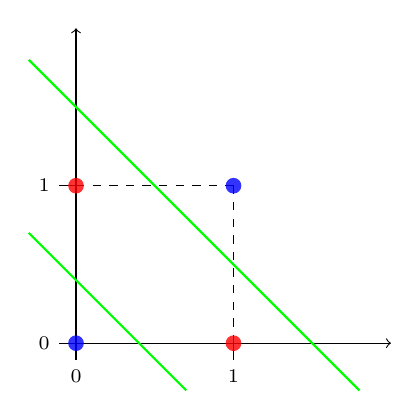
\begin{tikzpicture}[scale=2]
		
	 	% Axes
		\draw[->] (0,0) -- coordinate (x axis mid) (2,0);
	    \draw[->] (0,0) -- coordinate (y axis mid) (0,2);
		
		% Ticks
		\foreach \x in {0,...,1}
			\draw (\x,1pt) -- (\x,-3pt)
			 node[anchor=north] {\scriptsize\x};
		\foreach \y in {0,...,1}
			\draw (1pt,\y) -- (-3pt,\y)
			 node[anchor=east] {\scriptsize\y};
		
		\draw[dashed] (1,0) -- (1,1);
		\draw[dashed] (0,1) -- (1,1);
		
		\draw[thick, color=green] (0.7,-0.3) -- (-0.3,0.7);
		\draw[thick, color=green] (-0.3,1.8) -- (1.8,-0.3);
		
		\node[fill=blue, circle, inner sep=2pt, opacity=0.8] at (0,0) {};
		\node[fill=red, circle, inner sep=2pt, opacity=0.8] at (0,1) {};
		\node[fill=red, circle, inner sep=2pt, opacity=0.8] at (1,0) {};
		\node[fill=blue, circle, inner sep=2pt, opacity=0.8] at (1,1) {};
		
		
	\end{tikzpicture}
	\caption{Non separabilità lineare dell'operatore XOR}
\end{figure}

La convergenza del percettrone è garantita dal seguente teorema:

\begin{thm}[Teorema di Convergenza del Percettrone]
    Se il problema di classificazione è linearmente separabile allora la fase di apprendimento converge (termina) ad un'appropriata impostazione dei pesi in un numero finito di passi.
\end{thm}

Nella pratica non è dato sapere se un problema è o meno linearmente separabile. La convergenza si può comunque ottenere aggiustando i parametri del percettrone come ad esempio il numero di iterazioni o il fattore di apprendimento. In questo caso, tuttavia, la convergenza è artificiale.
% section percettrone_a_singolo_strato (end)



\section{Percettrone a più strati} % (fold)
\label{sec:percettrone_a_più_strati}
Come si è visto nei paragrafi precedenti il percettrone a singolo strato è limitato ai problemi linearmente separabili. Aggiungendo strati nascosti è possibile, tuttavia, rappresentare tutte le operazioni booleane incluso lo XOR. I percettroni multi-strato sono noti da molto tempo, ma gli algoritmi per l'apprendimento sono stati ideati solo recentemente (1986).\\

La rete di un percettrone multi-strato consiste in un insieme di ingressi (input layer), uno o più strati nascosti di neuroni (hidden layers) e un insieme di neuroni di uscita (output layer). Il segnale di input si propaga attraverso la rete in avanti da layer a layer.

\newpage

Una rete di questo tipo ha tre caratteristiche distintive:
\begin{itemize}
    \item ogni neurone include una \textbf{funzione di attivazione non lineare differenziabile }(ad es: funzione
sigmoidale);
    \item la rete contiene una o più strati nascosti (\textbf{hidden layers}) che non fanno parte né dell'input né
dell'output della rete;
    \item la rete ha un \textbf{alta connettività}.
\end{itemize}
In questa rete troviamo due tipi di segnali:
\begin{enumerate}
    \item \textbf{segnali di funzione: }un segnale di funzione è un segnale di input o stimolo che entra nel layer di input, si propaga in avanti attraverso gli strati nascosti per emergere al layer di uscita come segnale di output;
    \item \textbf{segnale di errore:} un segnale di errore ha origine nel layer di uscita e si propaga all'indietro attraverso la rete.
\end{enumerate}

Ogni neurone nascosto o d'uscita di un multilayer perceptron esegue due computazioni:
\begin{enumerate}
    \item la \textbf{computazione del segnale di funzione} espressa come funzione non lineare continua
di un segnale di input e dei pesi sinaptici associati al neurone;
    \item la \textbf{computazione di un vettore gradiente} necessario per aggiornamento dei pesi
sinaptici.
\end{enumerate}


\newpage

\begin{figure}[h!]
    \centering
    \includegraphics[width=10cm]{images/layers}
	\caption{Confronto tra diverse architetture di rete. Si osservi che ad ogni nuovo strato intermedio della rete, si ha una migliore classificazione delle forme che identificano le regioni delle due classi.}
\end{figure}


% section percettrone_a_più_strati (end)

\section{Previsione di serie temporali} % (fold)
\label{sec:previsione_di_serie_temporali}
Oltre ai problemi di classificazione, una rete neurale è in grado di affrontare anche altri tipi di problemi come ad esempio la previsione di una serie temporale \textbf{(time series prediction)}. Si tratta di un problema \emph{continuo} a differenza della classificazione che è, invece, \emph{discreto}.\\

Si consideri una sequenza $P$ di vettori o scalari che dipendono dal tempo $t$.
\begin{align*}
    P = \{x(t_0), x(t_1), \cdots, x(t_i - 1), x(t_i), x(t_i + 1), \cdots\}
\end{align*}
$t$ è un valore reale e $x(t)$ è un segnale continuo.\\

Per ottenere una serie $\{x[t]\}$ da un segnale continuo è necessario \emph{campionare} dal segnale in punti discreti. 

\newpage

Partendo da un tempo $t$ e campionando a ritroso, otteniamo la serie temporale $\{x[t], x[t-1], \cdots\}$. Lo scopo dell'analisi è di stimare $x$ a un tempo futuro.
\begin{align*}
    \hat{x}[t+s] = f(x[t], x[t-1], \cdots)
\end{align*}
Dove $s$ è noto come \emph{orizzonte della previsione}. Si tratta di un problema di approssimazione di una funzione e può essere risolto utilizzando una rete neurale a due strati. Il risultato è garantito dal seguente teorema:

\begin{thm}[Teorema dell'approssimazione universale]
    Una rete neurale multistrato feed-forward con un singolo strato nascosto, un percettrone, che contiene un numero finito di neuroni nascosti è un approssimatore universale di funzioni continue su sottoinsiemi compatti $\mathbb{R}^n$.
\end{thm}

% section previsione_di_serie_temporali (end)

% chapter problema_di_classificazione (end)
